\documentclass{report}
\usepackage[utf8]{inputenc}
\usepackage[T1]{fontenc}
\usepackage{CormorantGaramond}
\usepackage{fontspec}
\usepackage{geometry}
\usepackage[table]{xcolor}
\usepackage{tabularx}
\usepackage{graphicx}
\usepackage{mathtools}
\usepackage[bottom]{footmisc}
\usepackage[italian]{babel}
\usepackage{hyperref}
\usepackage{titlesec}
\usepackage{listings}
\usepackage{color}
\usepackage{graphicx}
\usepackage{xltabular}
\usepackage{fancyhdr}
\usepackage{pgf-pie}
\usepackage{float}

\renewcommand{\headrulewidth}{0.4pt}
\renewcommand{\footrulewidth}{0.4pt}

\lstset{ % General setup for the package
    basicstyle=\small\sffamily,
    numbers=left,
     numberstyle=\tiny,
    frame=tb,
    tabsize=4,
    columns=fixed,
    showstringspaces=false,
    showtabs=false,
    keepspaces,
    commentstyle=\color{red},
    keywordstyle=\color{blue}
}

\geometry{
a4paper,
total = {170mm, 240mm},
left = 20mm,
top = 20mm,
}

\setlength{\headheight}{33.60004pt}

\setlength{\parindent}{0em}
\setlength{\parskip}{0.7em}

\titlespacing{\section}{0pt}{0.7em}{0.5em}
\titlespacing{\subsection}{0pt}{0.7em}{0.5em}

\newcommand{\gassets}{../}

\renewcommand{\title}{
    Specifica architetturale

    \tiny Versione documento: \textit{V1.0.1}
}

\newcommand{\people}{
    \normalsize
    \begin{center}
        \begin{tabularx}{7cm}{l | X}            
            \textbf{Uso} & Esterno\\
            \textbf{Destinatario} & Committente\\
            & Cliente \\
        \end{tabularx}
    \end{center}
}

\fancypagestyle{plain}{%
    \fancyhead{} % clear all header fields
    \fancyhead[L]{\leftmark}
    \fancyhead[R]{\textit{SWEasabi} \includegraphics[height=30pt]{\gassets global-assets/img/loghi/SWEasabi_compact_logo.png}}
    \fancyfoot{} % clear all footer fields
    \fancyfoot[L]{\thepage}
    \fancyfoot[R]{Specifica architetturale}
}

\begin{document}

\pagestyle{fancy}

\fancyhead{} % clear all header fields
\fancyhead[L]{\leftmark}
\fancyhead[R]{\textit{SWEasabi} \includegraphics[height=30pt]{\gassets global-assets/img/loghi/SWEasabi_compact_logo.png}}
\fancyfoot{} % clear all footer fields
\fancyfoot[L]{\thepage}
\fancyfoot[R]{Specifica architetturale}



\input{\gassets global-assets/tex/header}
\thispagestyle{empty}
\clearpage
\pagenumbering{Roman}
\section{Registro delle modifiche}

\newcommand{\pzerozerootto}{
    \begin{center}
        \begin{tabularx}{\linewidth}{l | X}
            \textbf{Approvazione} & Peron Samuel\\
            \hline
            \textbf{Redazione}& Romano Davide\\
            \hline
            \textbf{Verifica} & Massarenti Alessandro\\
        \end{tabularx}
    \end{center}
}

\newcommand{\mzerozerootto}{
    \begin{itemize}
        \item Aggiunte sezioni progettazione logica all'appendice della specifica delle basi di dati, capitolo \ref{cap:appendice-basi-dati}.
    \end{itemize}
}

\newcommand{\vzerozerootto}{
    \hline
    0.0.8 & 21 lug 2023 & \mzerozerootto & \pzerozerootto\\
}
\newcommand{\pzerozerosei}{
    \begin{center}
        \begin{tabularx}{\linewidth}{l | X}
            \textbf{Approvazione} & Peron Samuel\\
            \hline
            \textbf{Redazione}& Romano Davide\\
            \hline
            \textbf{Verifica} & Massarenti Alessandro\\
        \end{tabularx}
    \end{center}
}

\newcommand{\mzerozerosei}{
    \begin{itemize}
        \item Aggiunta appendice della specifica delle basi di dati, capitolo \ref{cap:appendice-basi-dati}, con draft della struttura.
    \end{itemize}
}

\newcommand{\vzerozerosei}{
    \hline
    0.0.6 & 18 lug 2023 & \mzerozerosei & \pzerozerosei\\
}
\newcommand{\pzerozeroquattro}{
    \begin{center}
        \begin{tabularx}{\linewidth}{l | X}
            \textbf{Approvazione} & Romano Davide\\
            \hline
            \textbf{Redazione}& Alessandro Massarenti\\
            & Mattia Casarotto\\
            & Samuel Peron\\
            \hline
            \textbf{Verifica} & Michele Bonavigo\\
        \end{tabularx}
    \end{center}
}

\newcommand{\mzerozeroquattro}{
    \begin{itemize}
        \item Prima stesura dell'architettura del sistema di anagrafe, capitolo \ref{cap:microservizio-anagrafica};
    \end{itemize}
}

\newcommand{\vzerozeroquattro}{
    \hline
    0.0.4 & 14 giu 2023 & \mzerozeroquattro & \pzerozeroquattro\\
}





\newcommand{\pzerozerotre}{due
    \begin{center}
        \begin{tabularx}{\linewidth}{l | X}
            \textbf{Approvazione} & Romano Davide\\
            \hline
            \textbf{Redazione}& Alessandro Massarenti\\
            & Mattia Casarotto\\
            \hline
            \textbf{Verifica} & Samuel Peron\\
        \end{tabularx}
    \end{center}
}

\newcommand{\mzerozerotre}{
    \begin{itemize}
        \item Prima stesura dell'architettura generale del sistema, capitolo \ref{cap:architettura-generale};
    \end{itemize}
}

\newcommand{\vzerozerotre}{
    \hline
    0.0.3 & 07 giu 2023 & \mzerozerotre & \pzerozerotre\\
}





\newcommand{\pzerozerodue}{
    \begin{center}
        \begin{tabularx}{\linewidth}{l | X}
            \textbf{Approvazione} & Luca Pierobon\\
            \hline
            \textbf{Redazione}& Alessandro Massarenti\\
            & Michele Bonavigo\\
            \hline
            \textbf{Verifica} & Samuel Peron\\
        \end{tabularx}
    \end{center}
}

\newcommand{\mzerozerodue}{
    \begin{itemize}
        \item Prima stesura del sistema di autenticazione
    \end{itemize}
}

\newcommand{\vzerozerodue}{
    \hline
    0.0.2 & 06 giu 2023 & \mzerozerodue & \pzerozerodue\\
}





\newcommand{\pzerozerouno}{
    \begin{center}
        \begin{tabularx}{\linewidth}{l | X}
            \textbf{Approvazione} & Test\\
            \hline
            \textbf{Redazione}& Test\\
            & Test\\
            \hline
            \textbf{Verifica} & Test\\
        \end{tabularx}
    \end{center}
}
\newcommand{\mzerozerouno}{
    \begin{itemize}
        \item Prima stesura del documento e definzione struttura
    \end{itemize}
}

\newcommand{\vzerozerouno}{
    \hline
    0.0.1 & 15 mag 2023 & \mzerozerouno & \pzerozerouno\\
}





%Tabella
\begin{center}
    \begin{xltabular}{\linewidth}{|l|l|X|X|}
        \hline
        \textbf{Versione} & \textbf{Data} & \textbf{Modifica}& \textbf{Persone}\\
        \vzerozerootto
        \vzerozerosei
        \vzerozeroquattro
        \vzerozerotre
        \vzerozerodue
        \vzerozerouno
        \hline
    \end{xltabular}
\end{center}

\tableofcontents
\clearpage
\pagenumbering{arabic}
\chapter{Introduzione}

\section{Scopo del Documento}
Nel seguente documento viene illustrato in modo dettagliato la struttura e la composizione dei vari microservizi che compongo il prodotto. Il documento tratterà, in ordine, i seguenti punti:
\begin{itemize}
    \item WebApp;
    \item sistema di logging;
    \item sistema di illuminazione;
    \item sistema di anagrafica;
    \item sistema di autorizzazione.
\end{itemize}

\section{Scopo dell'architettura}
L'obiettivo di SWEasabi e dell'azienda ImolaInformatica S.p.A. è lo sviluppo di un sistema per l'ottimizzazione dell'illuminazione, il prodotto presenta differenti servizi che comunicano tra loro, ogni servizio ha un compito ben preciso e si occupa di una parte del sistema per questo necessità di una architettura ben definita e strutturata.
In questo documento verrà presentata l'architettura dei vari sistemi, i design pattern utilizzati e le tecnologie adottate.


\section{Glossario}
Per evitare ambiguità relative alle terminologie utilizzate è stato creato un documento denominato \href{https://github.com/SWEasabi/glossario/releases}{Glossario}.

Questo documento contiene tutti i termini specifici di settore utilizzati nei documenti, con le relative definizioni.

\section{Maturità del documento}
Il presente documento ha raggiunto un buon grado di maturità, in quanto sono state definite le tecnologie e i design pattern utilizzati per lo sviluppo del prodotto. Inoltre sono state definite le interazioni tra i vari servizi che compongono il prodotto.

\section{Riferimenti}
\subsection{Riferimenti Normativi}
\begin{itemize}
    \item \href{https://github.com/SWEasabi/norme-di-progetto/releases}{Norme di progetto};
    \item \href{https://www.math.unipd.it/~tullio/IS-1/2022/Progetto/C2.pdf}{capitolato d'appalto C2}.
\end{itemize}

\subsection{Riferimenti Informativi}
\begin{itemize}
    \item \href{https://github.com/SWEasabi/analisi-dei-requisiti/releases}{Analisi dei requisiti}
    \item \href{https://www.math.unipd.it/~rcardin/swea/2022/Software%20Architecture%20Patterns.pdf}{Software Architecture Patterns};
    \item \href{https://jwt.io/}{JSON Web Token website};
\end{itemize}
\chapter{Architettura generale del sistema} \label{cap:architettura-generale}

\section{Topologia generale} \label{sec:topologia_generale}

Per la definizione di questo sistema software è stato scelto di utilizzare un'architettura a microservizi, in quanto permette di avere un sistema scalabile e flessibile. Il pattern topologico scelto è quello REST.

Sono presenti all'interno del sistema due parti principali. Una parte è dedicata all'interazione con l'utente, l'altra parte è dedicata alla gestione dei dati e della logica di business, tra cui la comunicazione con i sistemi esterni quali lampioni, sensori e api meteo.

Ognuna delle responsabilità del sistema è stata suddivisa in un microservizio come segue:

\begin{itemize}
    \item \textbf{WebApplication}: è il microservizio che si occupa di gestire l'interazione con l'utente;
    \item \textbf{Anagrafica}: è il microservizio che si occupa di gestire i dati anagrafici dei lampioni, dei gruppi e delle aree in cui questi sono collocati;
    \item \textbf{Coordinazione}: è il microservizio che si occupa di gestire l'accensione e lo spegnimento dei lampioni secondo regole specifiche e utilizzando le informazioni provenienti dai sensori e da api varie per ottimizzare l'illuminazione;
    \item \textbf{Autenticazione}: è il microservizio che si occupa di gestire l'autenticazione degli utenti e di fornire i token necessari per l'accesso agli altri servizi;
    \item \textbf{logging}: è il microservizio che si occupa di gestire i log dei lampioni e dei sensori. Da questi, inoltre, vengono estratte informazioni necessarie per la gestione dell'illuminazione e più in generale aggregazioni di dati utli per l'analisi e la presentazione all'utente.
\end{itemize}

Possiamo definire queste responsabilità come dei componenti. Ognuno di questi componenti ha un'interfaccia ben definita e può essere sostituito con un altro componente che implementa la stessa interfaccia. Questo ci permette di utilizzare al massimo le pratiche di CICD.

I componenti dell'applicazione, le interfacce utilizzate ed esposte e le funzionalità fornite sono mostrate in figura \ref{fig:componenti_generali}.

\begin{figure}[ht]
    \centering
    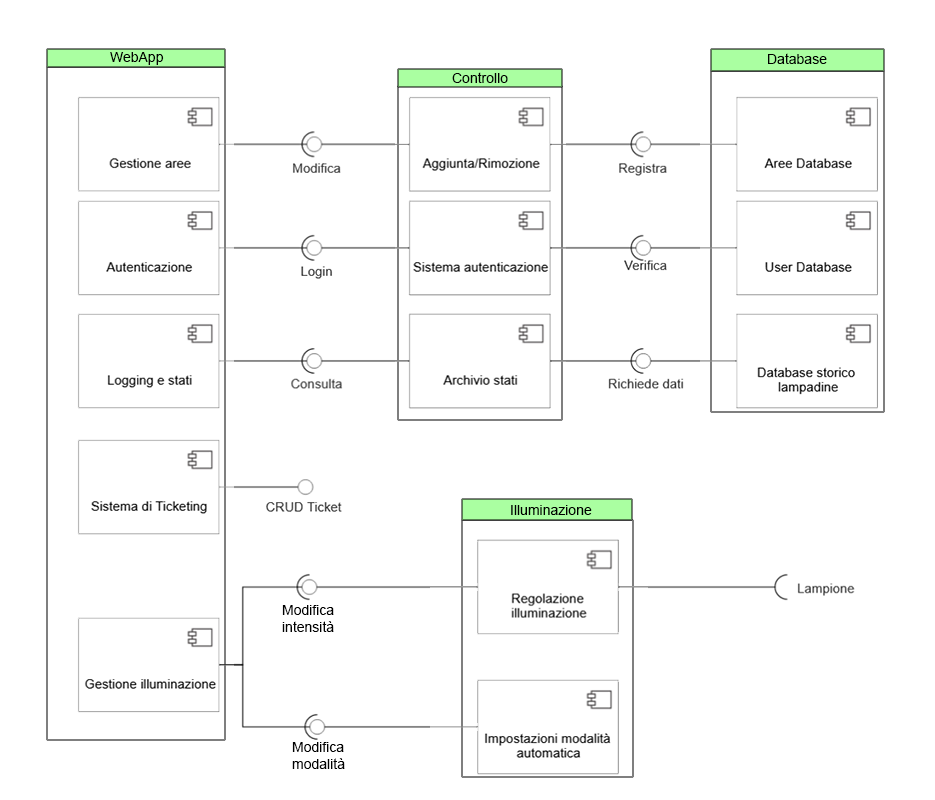
\includegraphics[width=\textwidth]{img/componenti_generali.png}
    \caption{Diagramma dei componenti del sistema generale}
    \label{fig:componenti_generali}
\end{figure}

\begin{figure}[ht]
    \centering
    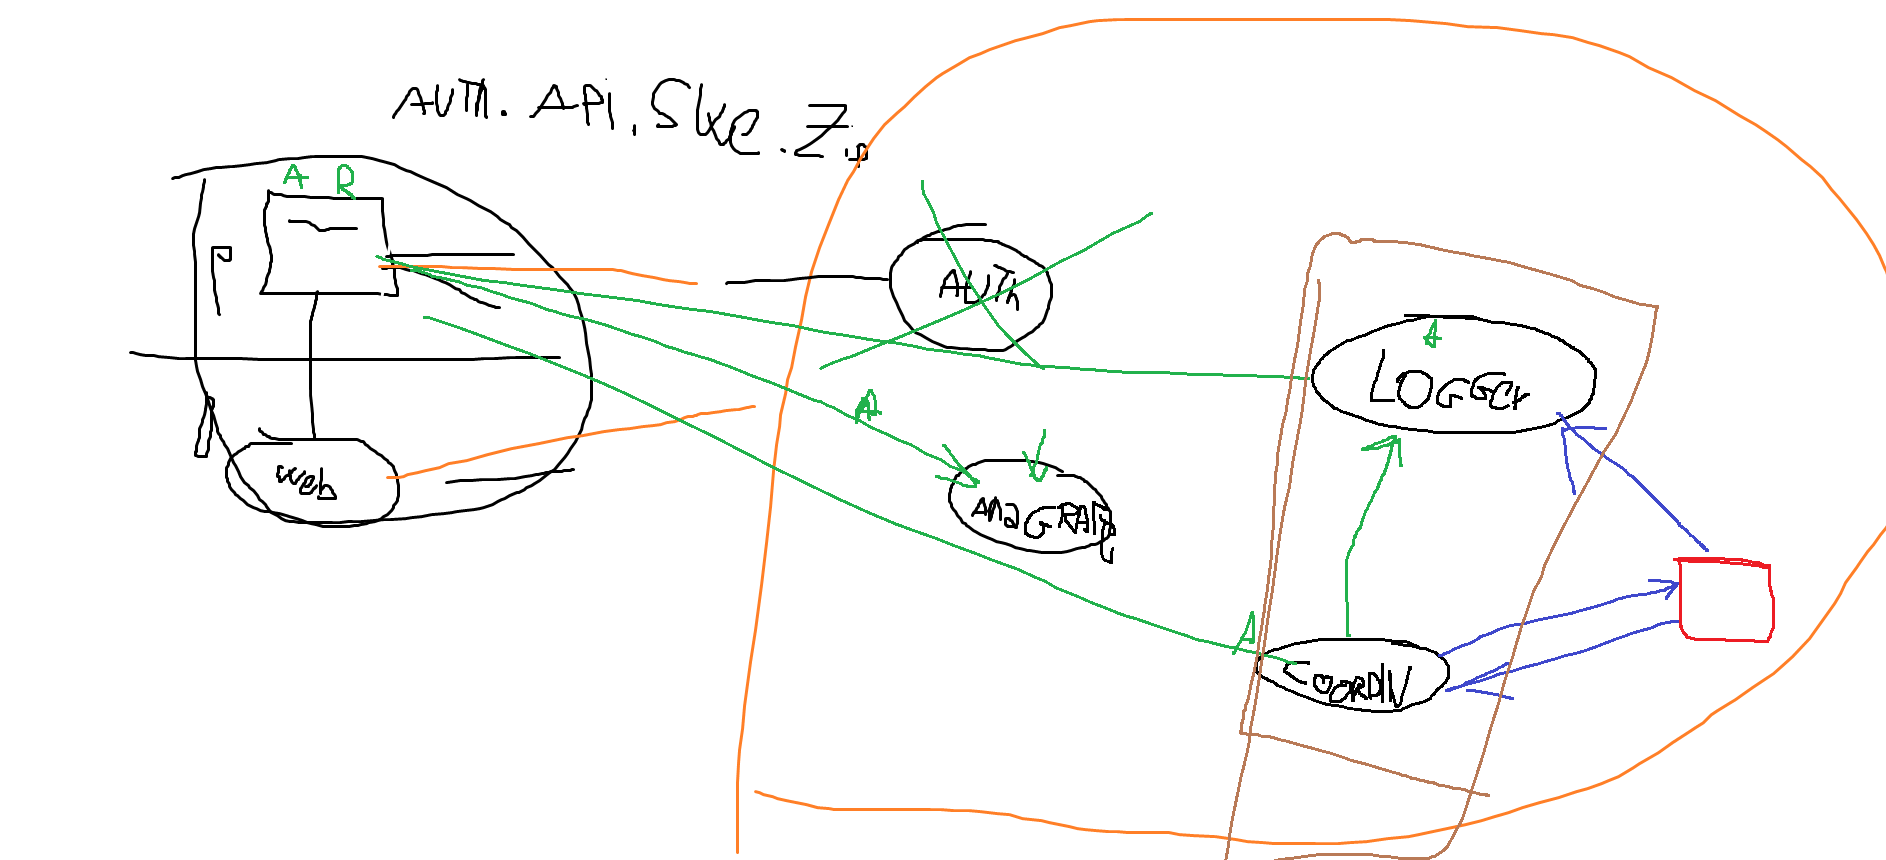
\includegraphics[width=\textwidth]{img/architettura_generale.png}
    \caption{Diagramma dell'architettura di sistema generale}
    \label{fig:architettura_generale}
\end{figure}

\section{User interface}

Come user Interface è stato scelto di utilizzare un'interfaccia web. Questa è stata scelta in quanto permette di avere un'interfaccia accessibile da qualsiasi dispositivo e non richiede l'installazione di software aggiuntivo. Inoltre, permette di avere un'interfaccia che può essere facilmente aggiornata e modificata.

Per l'implementazione é stato scelto di utilizzare il framework Angular.

La scelta di utilizzare una webapp come interfaccia utente risponde inoltre ai requisiti di vincolo: \textbf{RV\_01}, \textbf{RV\_02}, \textbf{RV\_03}, \textbf{RV\_04}, \textbf{RV\_05}.

In poche parole l'applicazione deve essere utilizzabile da mobile e dai maggiori browser nelle versioni più recenti. Questa è la definizione data dai requisiti sopra citati.

\section{Business backend e microservizi}

Il business backend è il componente che si occupa di gestire la logica di business dell'applicazione. Questo componente è composto dai microservizi citati precedentemente alla sezione \ref{sec:topologia_generale}.

La scelta di suddividere per responsabilità i microservizi serve a rispondere al requisito di vincolo \textbf{RV\_06}, ovvero che il sistema deve essere scalabile orizzontalmente. Questi Microservizi sono infatti inoltre anche gestiti in modo tale da rimanere stateless rispetto all'utente ed utilizzando per ciascuno un database separato. In caso di aumenti di carico del sistema è quindi semplicemente necessario aggiungere nuove istanze dei microservizi.

Avendo poi basi di dati ridotte ed utilizzando però DBMS relazionali per via della loro facilità d'utilizzo non è necessario dover creare complesse strategie di sharding per la suddivisione del carico.

\subsection{DNS}

Per la struttura posta dietro alla REST based architecture, ci sarà bisogno di una definizione di nomi di dominio. Questa definizione è necessaria per poter utilizzare le risorse specifiche di ogni microservizio senza utilizzare un livello intermedio di API.


\chapter{Webapp}\label{cap:webapp}

\section{Scopo del sistema}

La webapp permette all'utente di avere un interfaccia grafica con la quale gestire e monitorare lampioni,sensori ed aree inoltre permette di visualizzarne le informazioni relative.

\section{Requisiti coperti dal sistema}

\subsection{RV\_01}
RV\_01: l'applicazione deve essere visualizzabile su dispositivi mobile.

\subsection{RV\_02}
RV\_02: l'applicazione client deve poter essere utilizzata sulla versione più recente di Chrome (v. 110.0).

\subsection{RV\_03}
RV\_03: l'applicazione client deve poter essere utilizzata sulla versione più recente di Firefox (v. 110.0).

\subsection{RV\_04}
RV\_04: l'applicazione client deve poter essere utilizzata sulla versione più recente di Safari (v. 16.3).

\subsection{RV\_05}
RV\_05: l'applicazione client deve essere conforme almeno al livello AA delle WCAG.


\section{Descrizione del sistema}

La webapp è stata sviluppata utilizzando il framework AngularJS, il quale permette di creare applicazioni web single-page e di gestire le dipendenze tra le varie componenti dell'applicazione. Inoltre, è stato utilizzato il framework Bootstrap per la gestione della parte grafica. L'applicazione utilizza componenti di Angular, servizi e chiamate API per comunicare con il server. Le principali features dell'applicazione sono:
\begin{itemize}
    \item Visualizzazione lista di lampioni, sensori ed aree;
    \item Cambiare lo status dei lampioni e dei sensori;
    \item Aggiungere lampioni,sensori ed aree;
    \item Gestire caricamenti ed errori durante le chiamate API;
    \item Implementare l'autenticazione;
    \item Proteggere i collegamenti all'applicazione; 
\end{itemize} 

\section{Architettura del sistema}

La classe Model implementa tre interfacce che definiscono lo status di lampioni,sensori ed aree, queste definiscono la struttura e forniscono le proprietà per immagazinare informazioni quali status,identificativo e alias.
Le tre interfacce sono:
\begin{itemize}
    \item \textbf{LampStatus:} definisce lo stato di un lampione;
    \item \textbf{SensorStatus:} definisce lo stato di un sensore;
    \item \textbf{AreaStatus:} definisce lo stato di un'area;
\end{itemize}

La classe \textbf{Apiservice} definisce i metodi per effettuare le chiamate API e interagire con il server, questo servizio mette a dispozione i metodi per:
\begin{itemize}
    \item Ottenere la lista di lampioni, sensori ed aree;
    \item Ottenere lo stato di un lampione, sensore o area;
    \item Modificare lo stato di un lampione, sensore o area;
    \item Aggiungere un lampione, sensore o area;
    \item Ottenere i dati di un sensore;
    \item Ottenere i dati di un'area;
\end{itemize}

I componenti utilizzati dall'applicazione sono:
\begin{itemize}
    \item \textbf{LampsListComponent:} visualizza la lista di lampioni;
    \item \textbf{SensorsListComponent:} visualizza la lista di sensori;
    \item \textbf{AreasListComponent:} visualizza la lista di aree;
    \item \textbf{LampButtonComponent:} rappresenta un lampione della lista con il proprio stato e permette di modificarlo;
    \item \textbf{SensorButtonComponent:} rappresenta un sensore della lista con il proprio stato e permette di modificarlo;
    \item \textbf{AreaButtonComponent:} rappresenta un'area della lista con il proprio stato e permette di modificarlo;
\end{itemize}

L'applicazione presenta delle classi per l'utilizzo di altri microservizi:
\begin{itemize}
    \item \textbf{AuthService:} controlla l'autenticazione dell'utente;
    \item \textbf{AppService:} gestisce lo stato dell'applicazione mantenedo lo status di lampioni, sensori ed aree, questo servizio fornisce i metodi per l'aggiunta di nuovi dispositivi e comunica con l'API per ottenere dati,aggiornare gli status e gestire caricamenti ed errori;
\end{itemize}

La classe \textbf{AuthGuard} permette di proteggere i collegamenti all'applicazione, in questo modo l'utente non autenticato non può accedere alle pagine dell'applicazione.
\chapter{Microservizio anagrafica}\label{cap:microservizio-anagrafica}

\section{Scopo del sistema}

Il sistema di anagrafica si occupa di gestire le informazioni anagrafiche dei sensori, delle aree e dei lampioni. Gestisce questi raggruppamenti e si occupa di renderli persistenti su database.

\section{Requisiti coperti dal sistema}

\subsection{RF\_03}
RF\_03:deve essere possibile aggiungere nuovi sensori a sistema.

Questo microservizio, copre il requisito peristendo i dati anagrafici del sensore.

\subsection{RF\_08}
RF\_08:l'utente deve poter inserire la locazione geografica del sensore nel sistema.

Questo microservizio, copre il requisito peristendo i dati di locazione del sensore.

\subsection{RF\_09}
RF\_09:l'utente deve poter inserire il raggio di azione del sensore.

Questo microservizio, copre il requisito peristendo i dati di raggio di azione del sensore.

\subsection{RF\_10}
RF\_10:l'utente deve poter essere in grado di visualizzare quali aree sono illuminate in un dato momento

Questo microservizio, copre parte del requisito fornendo l'informazione di quali lampioni si trovano in una determinata area.



\section{Descrizione del sistema}

Il sistema principalmente fornisce le informazioni stoccate su base dati tramite un'interfaccia rest.
Questo è poi in grado di fornire i dati in forma aggregata, come ad esempio il numero di lampioni per area, o il numero di sensori per lampioni.

Per queste informazioni ha inoltre il compito e la responsabilità di tenere aggiornati i dati nel database.

\section{Architettura del sistema}

L'architettura base del sistema è in MVVM perché non è presente la necessità di multi input e multi output e un'architettura di altro tipo avrebbe aggiunto complessità inutile al sistema.

I componenti del programma sono quindi divisi in tre parti: Model, View e ViewModel.

\begin{figure}[h]
    \centering
    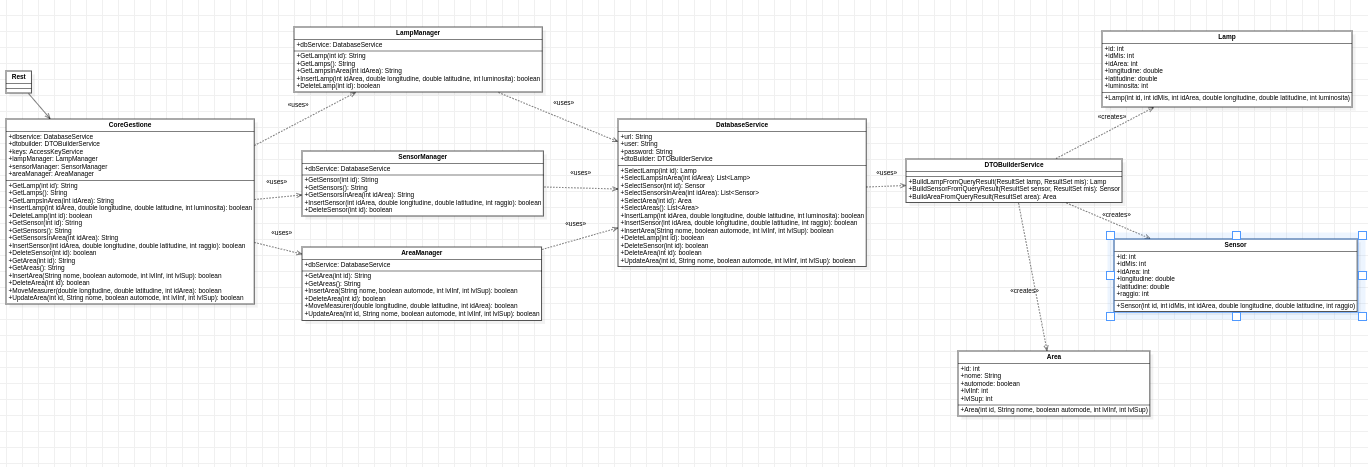
\includegraphics[width=\textwidth]{img/anagrafe_generale.png}
    \caption{Vista generale del sistema di anagrafe}
    \label{fig:general_anagrafe}
\end{figure}

\section{Model}
\begin{figure}[h]
    \centering
    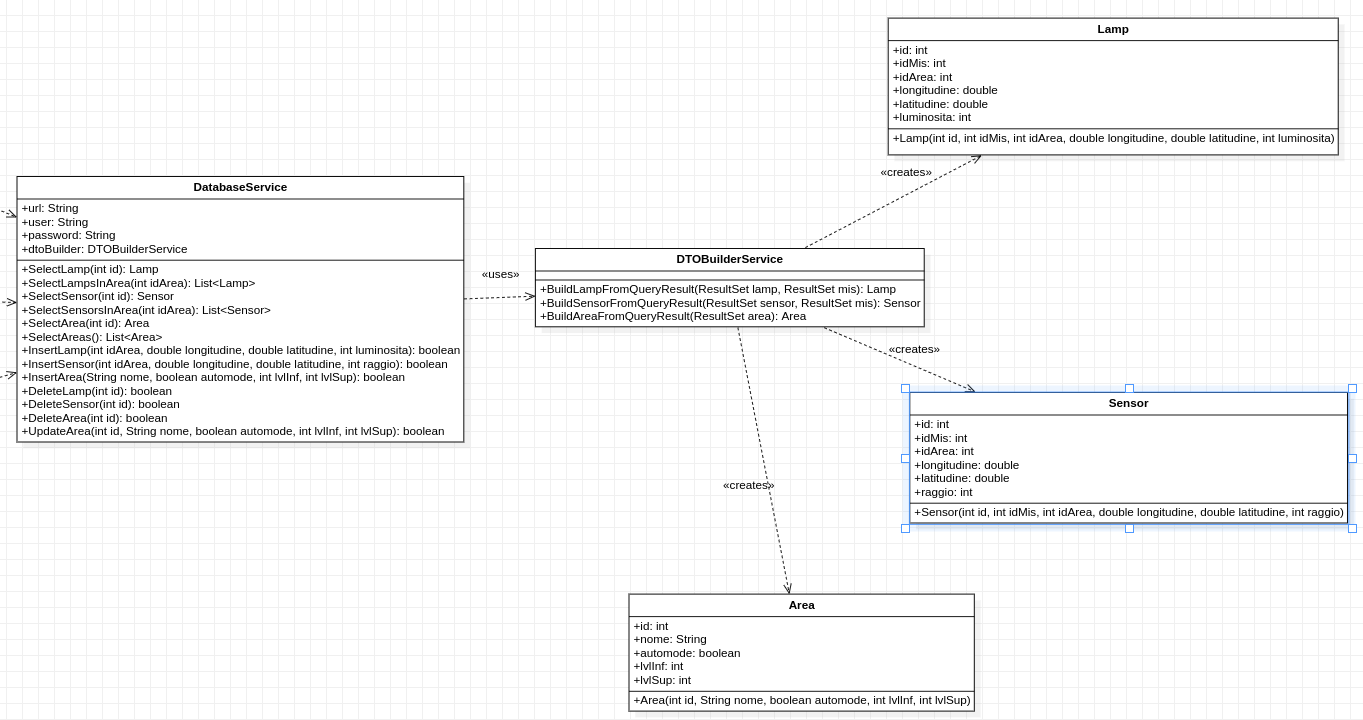
\includegraphics[width=\textwidth]{img/model_anagrafe.png}
    \caption{Diagramma delle classi del modello all'interno del sistema di anagrafe}
    \label{fig:model_anagrafe}
\end{figure}

\begin{itemize}
    \item \textbf{LampManager}: si occupa della gestione (ottenimento, inserimento, modifica o cancellazione) dei dati relativi ai lampioni nel database.
    \item \textbf{SensorManager:} si occupa della gestione (ottenimento, inserimento, modifica o cancellazione) dei dati relativi ai sensori nel database. 
    \item \textbf{AreaManager:} si occupa della gestione (ottenimento, inserimento, modifica o cancellazione) dei dati relativi alle aree nel database.
\end{itemize}

\section{Port Interfaccia REST}

L'interfaccia rest viene esposta all'esterno e permette di effettuare le operazioni discusse nelle sotto-sezioni successive.

\begin{itemize}
    \item GET /getLamp/id
    \item GET /getLampsInArea/idArea
    \item PUT /addLamp
    \item PUT /deleteLamp/id
    \item GET /getSensor/id
    \item GET /getSensorsInArea/idArea
    \item PUT /addSensor
    \item PUT /deleteSensor/id
    \item PUT /moveMeasurer/idMeasurer
    \item GET /getArea/id
    \item GET /getAreaList
    \item PUT /addArea
    \item PUT /updateArea/id
    \item PUT /deleteArea/id
\end{itemize}

\subsection{ GET /getLamp/id}

GetLamp permette di ottenere tutti i dati relativi a un lampione. L'utente deve fornire l'id del lampione in questione.

Il sistema risponderà con un JSON contenente tutti i dati relativi al lampione richiesto.

\subsection{ GET /getLampsInArea/idArea}

GetLampsInArea permette di ottenere i dati relativi a tutti i lampioni in un'area. L'utente deve fornire l'id dell'area della quale si desidera visualizzare i lampioni.

Il sistema risponderà con un JSON contenente tutti i dati relativi ai lampioni presenti in quell'area.

\subsection{ PUT /addLamp}

AddLamp permette di inserire nel database un nuovo lampione. All'utente è richiesto di fornire i dati relativi al lampione da inserire in un JSON che viene inviato al sistema.

Il sistema risponderà con un boolean ad indicare se l'operazione è andata a buon fine o meno.

\subsection{ PUT /deleteLamp/id}

DeleteLamp permette di eliminare dal database un lampione. L'utente deve fornire al sistema l'id del lampione da eliminare.

Il sistema procede poi a tentare di eliminare il lampione, rimuovendo prima il riferimento al misuratore, e ritorna un boolean positivo in caso di successo, negativo in caso di fallimento.

\subsection{ GET /getSensor/id}

GetSensor permette di ottenere tutti i dati relativi a un sensore. L'utente deve fornire l'id del sensore in questione.

Il sistema risponderà con un JSON contenente tutti i dati relativi al sensore richiesto.

\subsection{ GET /getSensorsInArea/idArea}

GetSensorsInArea permette di ottenere i dati relativi a tutti i sensorioni in un'area. L'utente deve fornire l'id dell'area della quale si desidera visualizzare i sensorioni.

Il sistema risponderà con un JSON contenente tutti i dati relativi ai sensorioni presenti in quell'area.

\subsection{ PUT /addSensor}

AddSensor permette di inserire nel database un nuovo sensore. All'utente è richiesto di fornire i dati relativi al sensore da inserire in un JSON che viene inviato al sistema.

Il sistema risponderà con un boolean ad indicare se l'operazione è andata a buon fine o meno.

\subsection{ PUT /deleteSensor/id}

DeleteSensor permette di eliminare dal database un sensore. L'utente deve fornire al sistema l'id del sensore da eliminare.

Il sistema procede poi a tentare di eliminare il sensore, rimuovendo prima il riferimento al misuratore, e ritorna un boolean positivo in caso di successo, negativo in caso di fallimento.

\subsection { PUT /moveMeasurer/id}

MoveMeasurer permette di spostare un misuratore (che può essere un lampione o un sensore) da un'area a un'altra. L'utente deve fornire l'id del misuratore da spostare e un JSON contenente le nuove coordinate e l'area dove va inserito.

Il sistema ritorna infine un boolean positivo in caso di successo, negativo in caso di fallimento.


\section{ViewModel}

\section{View}



\chapter{Sistema di coordinazione}\label{cap:sistema-coordinazione}

\section{Scopo del sistema}
Il sistema di coordinazione è il componente che si occupa di gestire i lampioni, regolandone l'accensione e lo spegnimento in base alle informazioni che ha a disposizione.\\

Tramite algoritmi sofisticati, il sistema di coordinazione è in grado di gestire l'illuminazione in modo efficiente.

\subsection{Requisiti coperti dal sistema}

\subsubsection{RF\_05}

RF\_05: Il sistema deve accendere un'area per un lasso di tempo preconfigurato quando rileva persone in prossimità dello stesso.

\subsubsection{RF\_06}

RF\_06: Il sistema deve riportare l'intensità luminosa dell'area al valore di default una volta passato il tempo impostato.

\subsubsection{RF\_19}

RF\_19: Il sistema deve essere in grado di ricevere informazioni dal sensore in modalità push.

\section{Descrizione del sistema}

Il sistema utilizza molteplici paradigmi. L'architettura generale è di tipo esagonale.

Il programma eseguirà azioni quando attivato da eventi esterni, quali l'arrivo di un nuovo stato da MQTT oppure l'arrivo di una richiesta da parte dell'utente collegato alla webapp\footnote{Si veda sezione \ref{cap:webapp}}.

Le componenti principali saranno:

\begin{itemize}
    \item \textbf{Porta ricevente MQTT}: si occupa di ricevere i messaggi da MQTT e di inoltrarli al sistema ad eventi;
    \item \textbf{Interfaccia REST}: si occupa di ricevere le richieste degli utenti e di inoltrarle al sistema ad eventi;
    \item \textbf{Pila di payload}: È una pila contenente i payload di dati da analizzare;
    \item \textbf{Algoritmo di analisi}: Dato un payload si occupa di analizzarlo e di generare un nuovo stato;
\end{itemize}

La pila di Payload usa il paradigma del \textbf{Producer-Consumer}, in cui il produttore è la porta ricevente, mentre il consumatore è l'algoritmo di analisi.

È poi presente un database\footnote{Vedi sezione relativa al database e alla sua progettazione \ref{cap:db-sistema-coordinatore}} al quale il sistema si connette, per mantenere gli stati anche in caso di reboot del sistema.

Inoltre, se il programma farà comunque del caching dei dati, sarà comunque nel database che verranno depositati i dati quando la cache diventa troppo grande.

\section{Architettura del sistema}

Il sistema è composto da un'interfaccia REST, un'interfaccia MQTT, un collegamento ad un db e un algoritmo di analisi.

\subsection{Entità del sistema}

\begin{itemize}
    \item \textbf{AreaAnagrafica}: Contiene le informazioni relative ad un'area, quali la posizione, il nome, il tipo di illuminazione, ecc.
    \item \textbf{LampAnagrafica}: Contiene le informazioni relative ad un lampione, quali la posizione, il nome, il tipo di illuminazione, ecc.
    \item \textbf{Misuratore}:
    \item \textbf{SensoreAnagrafica}: Contiene le informazioni relative ad un sensore, quali la posizione, il nome, il tipo di sensore, ecc.
\end{itemize}

\subsection{Classi legate al database}

Il database viene gestito come repository, e ognuna delle entità viene gestita come tale.

Le classi relative ai repository sono:

\begin{itemize}
    \item \textbf{AreaRepository}: Fornisce l'accesso al database per le aree;
    \item \textbf{LampRepository}: Fornisce l'accesso al database per i lampioni;
    \item \textbf{MisuratoreRepository}: 
    \item \textbf{SensoreRepository}: Fornisce l'accesso al database per i sensori;
\end{itemize}

Le classi sopra descritte sono visibili in figura \ref{fig:coordinazione_db}

\begin{figure}[h]
    \centering
    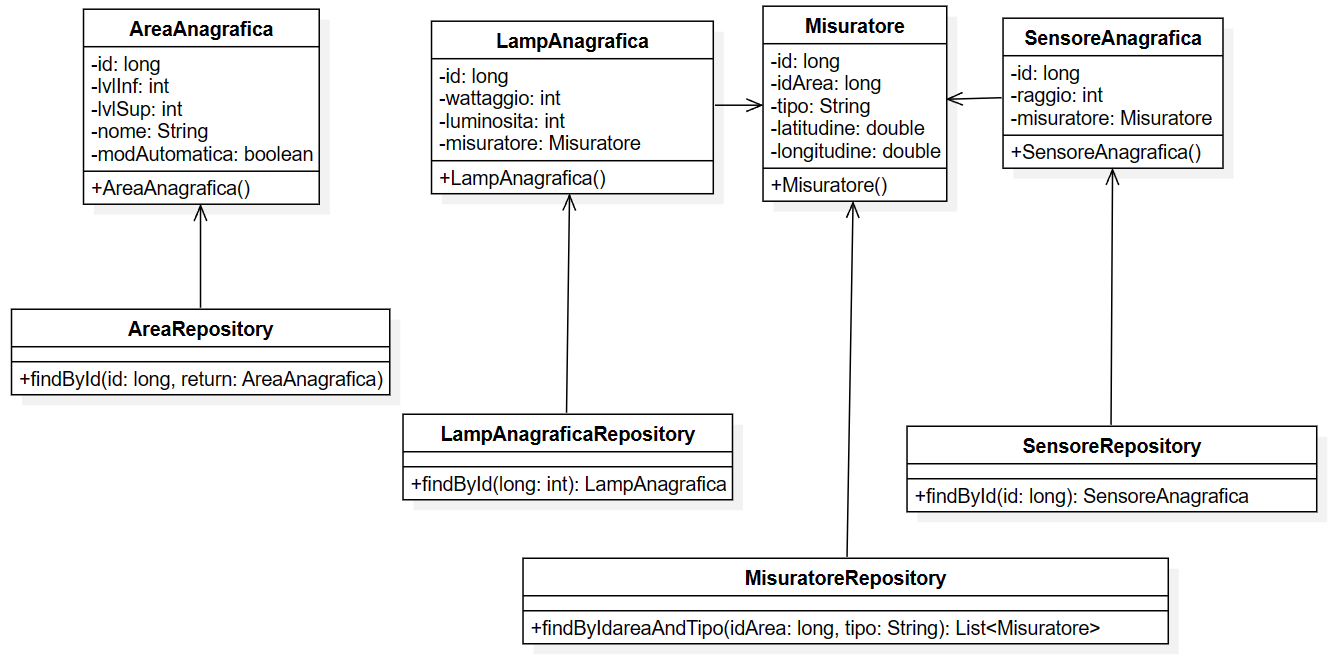
\includegraphics[width=\textwidth]{img/illuminazione_repository.png}
    \caption{Diagramma delle classi relative ai repository e al sistema connesso al database}
    \label{fig:coordinazione_db}
\end{figure}

Queste classi effettuano le operazioni sul db tramite JPA.

\subsection{Classi di configurazione}

La classe \textbf{Beanconfig} contiene tutti i bean di Spring relativi alla configurazione per mqtt e per il database.

\subsection{Classi legate ad MQTT}

Per la gestione di MQTT sono presenti le seguenti classi visibili in figura \ref{fig:coordinazione_mqtt}

\begin{figure}[h]
    \centering
    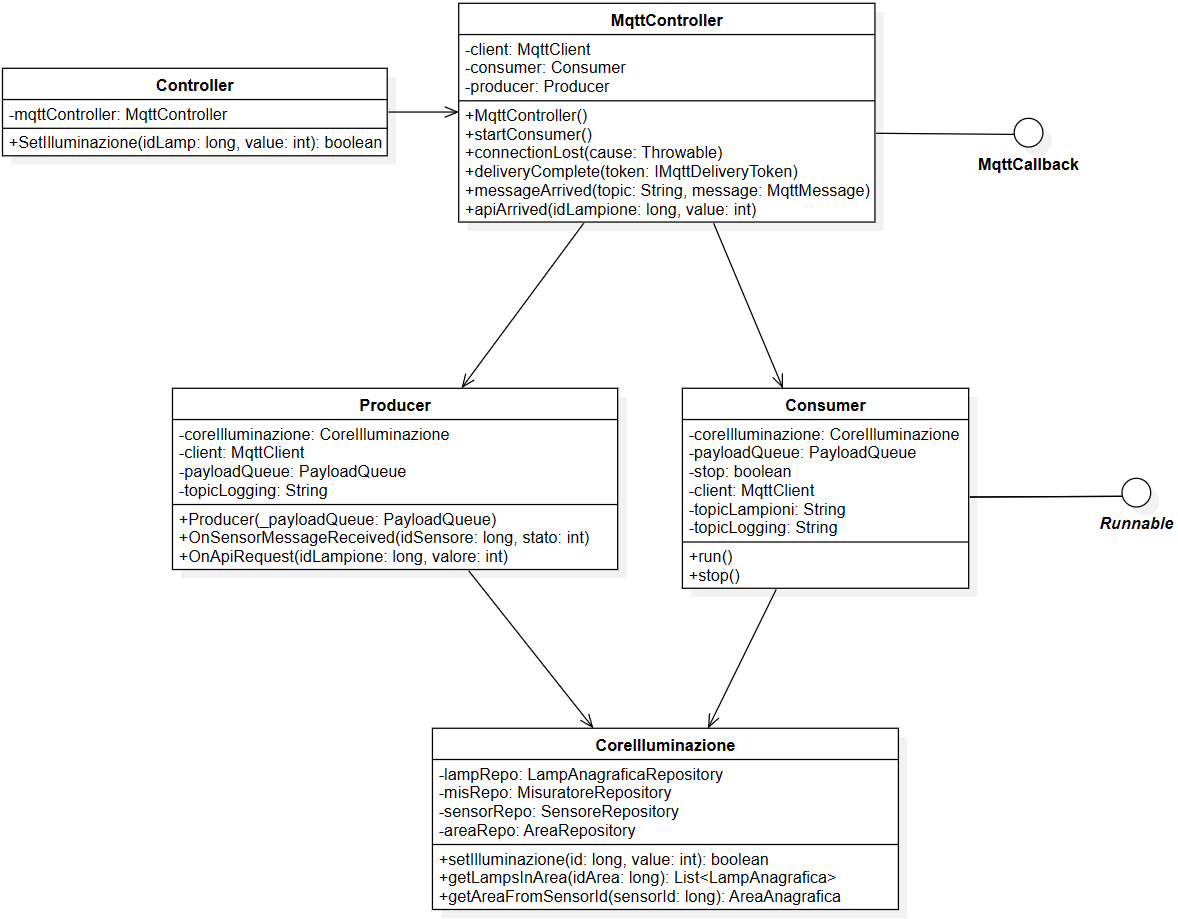
\includegraphics[width=\textwidth]{img/illuminazione_mqtt.png}
    \caption{Diagramma delle classi relative alla parte mqtt del sistema di coordinazione}
    \label{fig:coordinazione_mqtt}
\end{figure}


\begin{itemize}
    \item \textbf{MqttController}: Si occupa di gestire la ricezione dei messaggi da MQTT e di inoltrarli al sistema ad eventi;
    \item \textbf{Producer}: Questa classe rimane in ascolto delle rilavazioni MQTT, quando dal topic sensore arriva un cambiamento, questo viene segnalato al logging\footnote{Il logging poi loggerà l'informazione}. In ultimo genera un payload e lo aggiunge alla coda dei payload da processare;
    \item \textbf{Consumer}: Quando vede che la coda dei payload non è vuota raccoglie le operazioni da fare, analizza lo stato e modifica la luminosità dei lampioni via mqtt, inoltre aggiorna il database con il nuovo stato;
\end{itemize}

\subsubsection{Payloads}

I payloads sono un oggetto che contiene le informazioni necessarie per l'analisi e la modifica dello stato di illuminazione.

Queste classi vengono descritte nell'immagine \ref{fig:coordinazione_payload}.

\begin{figure}[h]
    \centering
    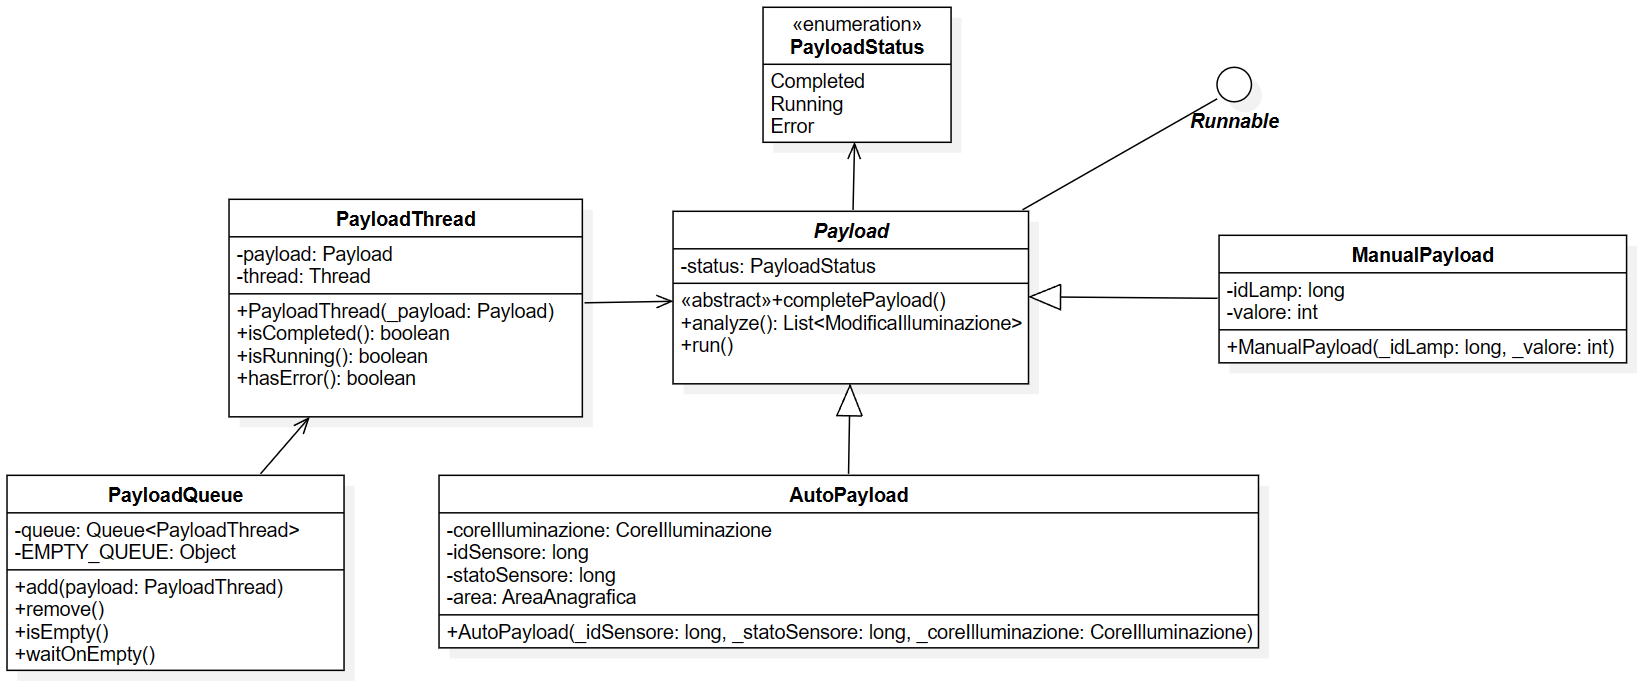
\includegraphics[width=\textwidth]{img/illuminazione_payload.png}
    \caption{Diagramma delle classi relativa ai payloads}
    \label{fig:coordinazione_payload}
\end{figure}

\paragraph{Payload} è un'interfaccia che contiene i metodi comuni a tutti i payloads.

\paragraph{PayloadQueue} è una coda di payload, che contiene i payload da processare.

\paragraph{PayloadThread} è un thread che si occupa di processare i payload.

\paragraph{PayloadStatus} è un enum che contiene i possibili stati dei payload.

\paragraph{PayloadManual} è un payload che contiene le informazioni per un'analisi manuale.

\paragraph{PayloadAuto} è un payload che contiene le informazioni per un'analisi automatica.

I payload manuali e automatici sono thread che fanno le loro operazioni in parallelo, controllano se c'è da modificare uno stato e in caso positivo preparano le informazioni per il consumer.

\chapter{Sistema di autenticazione}


\section{Scopo del sistema}

Il sistema di autenticazione ha lo scopo di gestire le richieste di autenticazione da parte degli utenti e di fornire un token di sessione valido per l'accesso alle risorse protette.

\section{Descrizione del sistema}

Il sistema di autenticazione è definito da un microservizio che espone un'interfaccia REST per la gestione delle richieste di autenticazione degli utenti. Il microservizio è inoltre responsabile della generazione e della validazione dei token di sessione.

I token di sessione utilizzati sono del tipo JWT (JSON Web Token) e sono composti da tre parti separate da un punto. La prima parte contiene le informazioni relative all'algoritmo di hashing utilizzato per la firma del token, la seconda parte contiene le informazioni relative all'utente autenticato e la terza parte contiene la firma del token.

\section{Architettura del sistema}

Il sistema utilizza un'architettura esagonale, in cui il core del sistema si occupa della business logic ed offre:
\begin{itemize}
    \item Generazione dei JWT;
    \item Refresh dei JWT;
    \item Autenticazione degli utenti.
\end{itemize}

\begin{figure}[H]
    \centering
    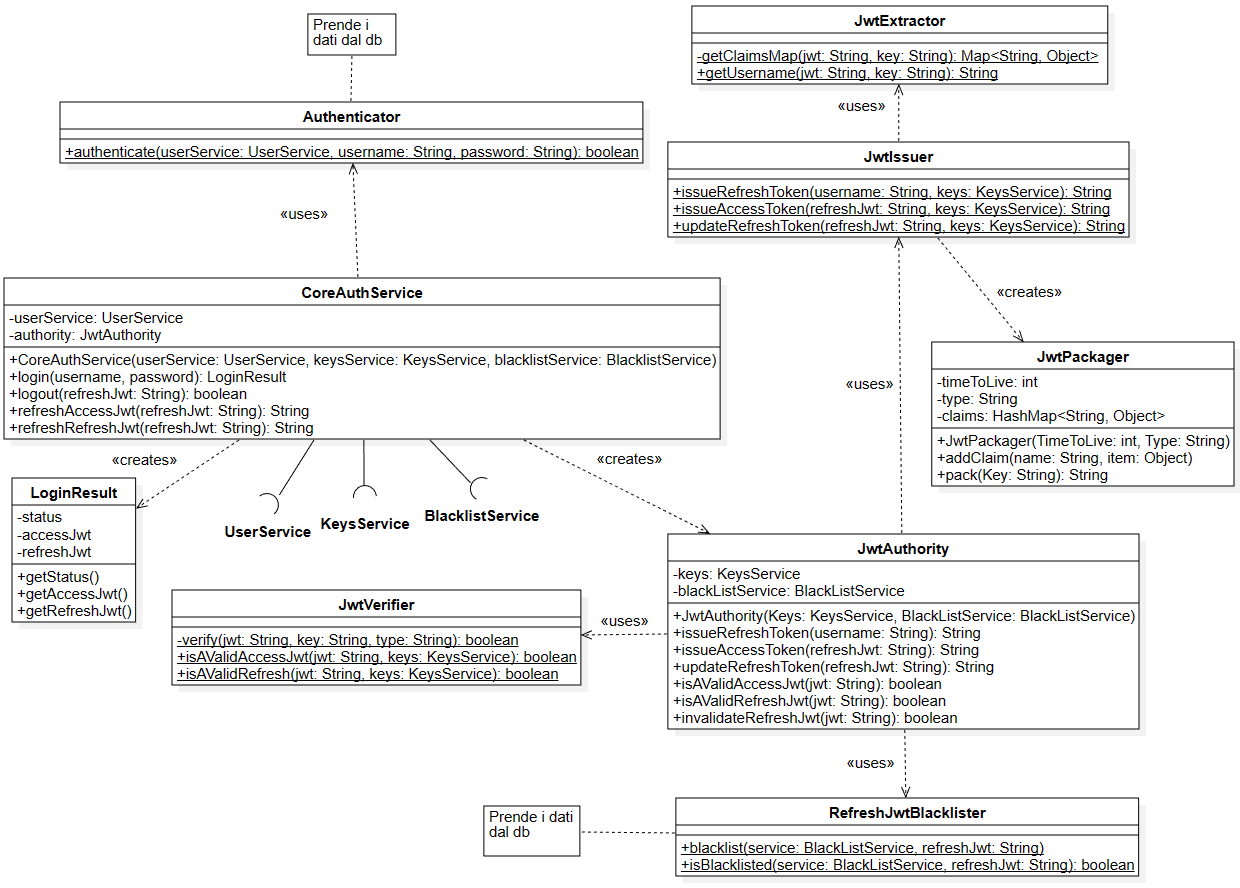
\includegraphics[width=\textwidth]{img/classi_auth.png}
    \caption{Diagramma delle classi del sistema di autenticazione}
\end{figure}

Il sistema offre poi un'interfaccia di tipo REST, e si connette sempre tramite l'utilizzo del sistema a porte ad un Database per la memorizzazione dei dati.

\subsection{I JWT}

Il sistema generale è pensato per utilizzare due tipologie di Token. Viene utilizzato un token di autorizzazione, che viene utilizzato per l'autenticazione e per l'accesso alle risorse protette degli altri microservizi e un token di refresh, che viene utilizzato per la generazione di un nuovo token di autorizzazione.

Ognuno dei microservizi del sistema accetta come valido un token generato da questo microservizio. Non accetterà però come valido un token di refresh.

Il token di refresh viene infatti riconosciuto solamente da questo sistema.

Il token di refresh ha durata di 2h, mentre il token di autorizzazione ha durata di 10 minuti.

\section{Interfaccia REST}

L'interfaccia rest viene esposta all'esterno e permette di effettuare le operazioni discusse nelle sotto-sezioni successive.

\subsection{Autenticazione}

POST /auth/login

\chapter{Sistema di logging}\label{cap:microservizio-logging}

\section{Scopo del sitema}

Il sistema di logging serve per mantenere uno storico dei cambiamenti di stato e valore dei vari dispositivi, in modo da poterli consultare in un secondo momento. 

\section{Requisiti del sistema}

\subsection{RF\_23}

RF\_23: L'utente deve essere in grado di visualizzare gli stati dei dispositivi in un certo periodo di tempo.

Questo microservizio, copre il requisito memorizzando gli stati dei dispositivi in un database.

\section{Descrizione del sistema}
Il sistema permette di leggere i dati storici degli stati dei dispositivi tramite un interfaccia rest. Rende quindi possibile la visione di un insieme di log con diverse opzioni, ad esempio in un certo periodo di tempo o gli ultimi n log.

\section{Architettura del sistema}

Il sistema è composto da un'interfaccia REST e un insieme di classi che si occupano di leggere i dati dal database.
Il servizio nasce molto semplice e per questo motivo non è stato ritenuto necessario l'utilizzo di un'architettura più complessa e strutturata.

\begin{figure}[ht]
    \centering
    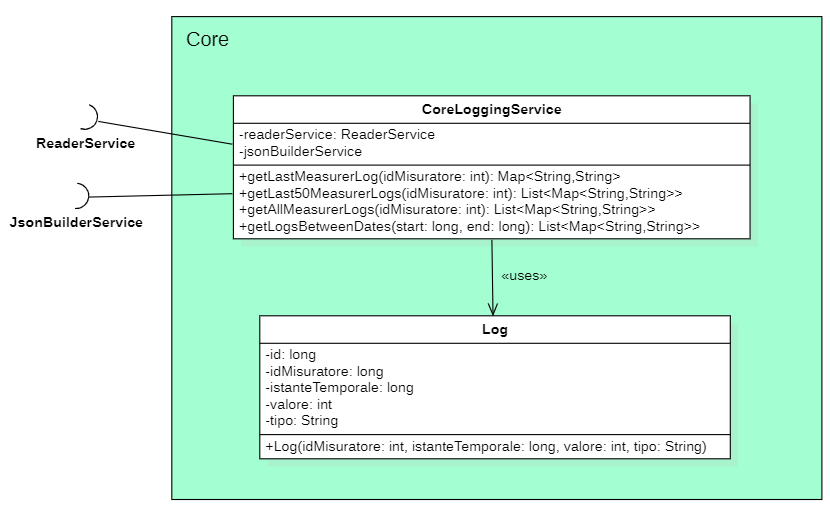
\includegraphics[width=0.6\textwidth]{img/classi_logging.png}
    \caption{Vista generale del sistema di logging}
    \label{fig:general_logging}
\end{figure}

\section{Repository}
Il LogRepository è un'interfaccia repository JPA ed esegue fisicamente le operazioni sul database.

\section{Servizi}

I servizi sono in generale le interfacce ad alto livello delle funzionalità del sistema. Sono composti da classi che si occupano di gestire le richieste e di fornire i dati richiesti.

\subsection{ReaderService}
ReaderService si occupa di leggere e fornire i dati dei log dal database in base alla richiesta.

ReaderService viene realizzata in localReaderService per i test. Invece per connettersi al db viene utilizzata la classe DatabaseReaderService.

\section{Core}
Il core è il nucleo del sistema ed in generale si pone come facade per tutti i servizi che si trovano all'interno del microservizio. Questa classe si occupa di gestire le richieste e di fornire i dati richiesti.
Principalmente questa classe viene utilizzata dall'interfaccia REST.

\section{Log}
La classe Log viene utilizzata per trasferire le informazioni tra le varie classi ed è costruito da logrepository quando fa operazioni sul database e deve ritornarne uno.

\section{JsonBuilderService}
Si occupa di creare i JSON da ritornare all'interfaccia REST a partire dai log.

\section{ Config}
La classe Config genera i bean che servono alle altre classi per funzionare.



\section{Interfaccia REST}

\begin{figure}[ht]
    \centering
    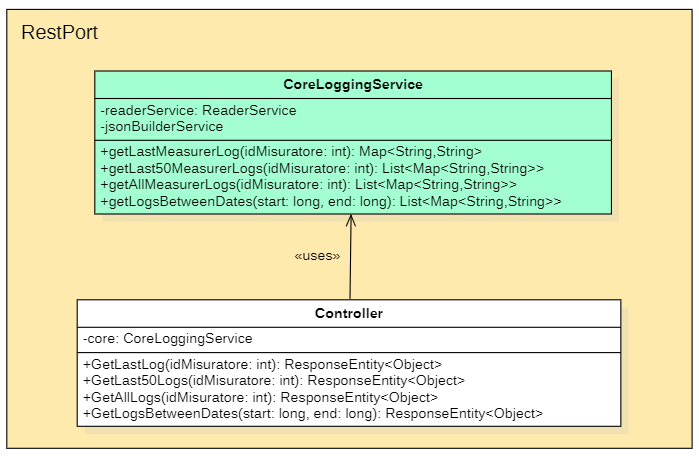
\includegraphics[width=0.8\textwidth]{img/classi_logging_port_rest.png}
    \caption{Vista delle classi che si occupano dell'interfaccia rest}
    \label{fig:rest_logging}
\end{figure}

\begin{itemize}
    \item GET /log/last/{idMisuratore}
    \item GET /log/last50/{idMisuratore}
    \item GET /log/all/{idMisuratore}
    \item GET /log/dates/{start}/{end}
\end{itemize}

\subsection{GET /log/last/{idMisuratore}}
Get /log/last/{idMisuratore} ritorna l'ultimo log del dispositivo con id idMisuratore.

\subsection{GET /log/last50/{idMisuratore}}
Get /log/last50/{idMisuratore} ritorna gli ultimi 50 log del dispositivo con id idMisuratore.

\subsection{GET /log/all/{idMisuratore}}
Get /log/all/{idMisuratore} ritorna tutti i log del dispositivo con id idMisuratore.

\subsection{GET /log/dates/{start}/{end}}
Get /log/dates/{start}/{end} ritorna tutti i log compresi tra start e end.






%Appendici
\appendix
\chapter{Specifica delle basi di dati} \label{cap:appendice-basi-dati}

\section{Base di dati sistema anagrafe}

\subsection{Abstract}

L'obiettivo è sviluppare un servizio che tenga ordinati e renda sempre disponibili tutte le informazioni relative a nomi, gruppi, peculiarità di ognuno dei sensori, delle aree, e dei lampioni. 

Queste informazioni sono particolarmente utili per contestualizzare ognuna delle componenti {\it{hardware}} del sistema.

\subsection{Analisi dei requisiti}

\subsection{Progettazione concettuale}

\subsection{Progettazione logica}

\subsubsection{Eliminazione delle generalizzazioni}

\paragraph{Misuratore}

Per evitare di accorpare le entità Sensore e Lampione nell'entità padre Misuratore, creando così dei campi NULL, è stato deciso di risolvere la generalizzazione mantenendo le tre entità inserendo le relazioni tra le entità figlie e l'entità padre.

\subsubsection{Modifiche, aggiunte e chiarimenti alle chiavi}

Tutte le chiavi primarie sono definite utilizzando le chiavi della progettazione concettuale, tranne nei seguenti casi.

\paragraph{Sensore} Diventando il Sensore un'entità a sé stante, vengono aggiunte una chiave primaria ed una chiave esterna che indica il Misuratore a cui fa riferimento.

\paragraph{Lampione} Diventando il Lampione un'entità a sé stante, vengono aggiunte una chiave primaria ed una chiave esterna che indica il Misuratore a cui fa riferimento.

\subsubsection{Schema concettuale ristrutturato - Schema Logico}

\begin{center}
    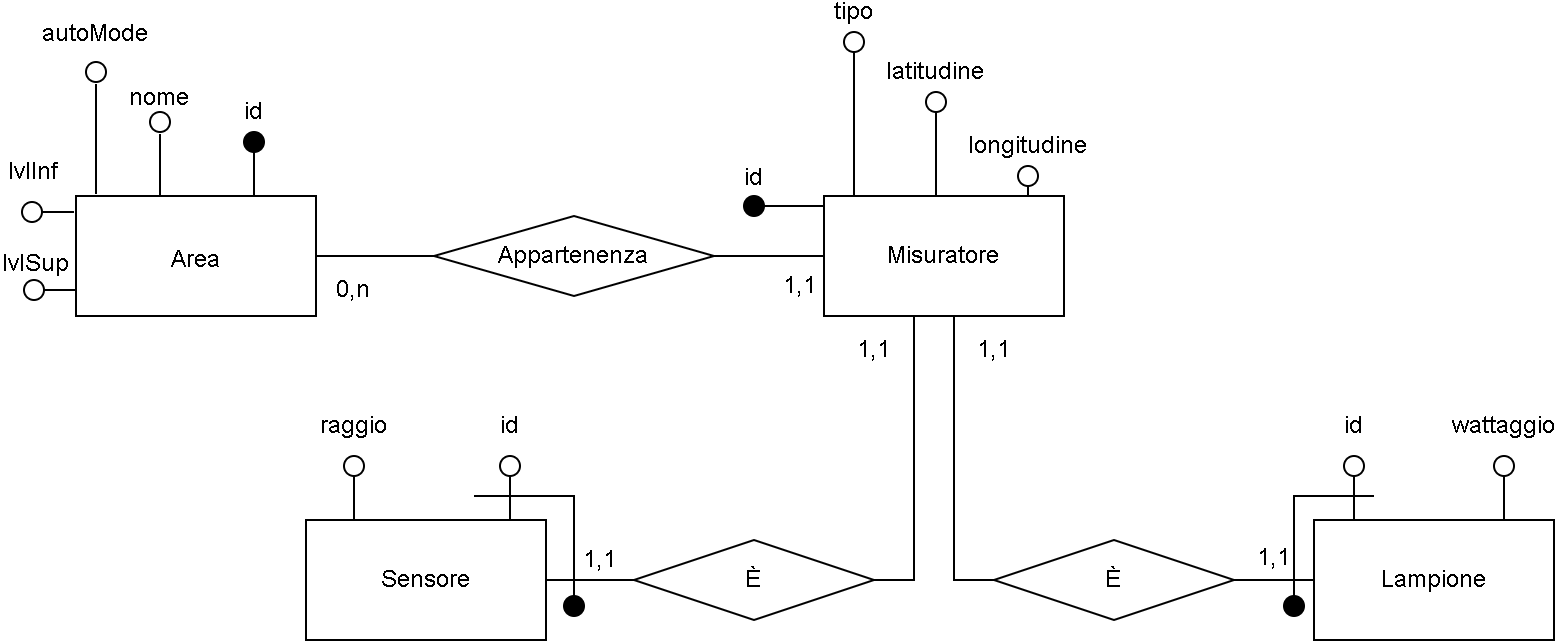
\includegraphics[width=12cm]{contenuti/specifica-basi-dati/img-sbd/anagrafica_logico.png}
\end{center}

\subsubsection{Descrizione schema relazionale}

Per questione di compatibilità con il DBMS alcuni nomi di attributi entità e relazioni sono stati normalizzati, utilizzando il camelCase, togliendo gli accenti, accorciando i nomi molto lunghi e con altre piccole accortezze.
La chiave primaria è indicata in \textbf{grassetto}, le chiavi esterne sono indicate con la \underline{sottolineatura}.

\textit{Area}(\textbf{id}, nome, autoMode, lvlInf, lvlSup) \\
\textit{Misuratore}(\textbf{id}, \underline{idArea}, tipo, latitudine, longitudine) \\
\textit{Sensore}(\textbf{id}, \underline{idMisuratore}, raggio) \\
\textit{Lampione}(\textbf{id}, \underline{idMisuratore}, luminosita)

\subsubsection{Vincoli di integrità referenziali}

\textbf{Sensore}.idMisuratore -> \textit{Misuratore}.id \\
\textbf{Lampione}.idMisuratore -> \textit{Misuratore}.id

\subsubsection{Check e constraint}

\paragraph{Area} In \textbf{Area} è attivato un check che controlla che il valore del livello inferiore sia sempre minore del valore del livello superiore.
\section{Base di dati sistema coordinazione}\label{sec:sbd-sistema-coordinazione}

\subsection{Abstract}

L'obiettivo è quello di sviluppare un sistema che coordini e decida quando illuminare o non illuminare specifiche zone. Questo sistema dovrà tenere traccia di tutte le informazioni relative allo stato attuale dei lampioni.

Il sistema si collegherà ad altre componenti esterne, utilizzando algoritmi proprietari, e deciderà quando effettuare cambiamenti di stato. Si consiglia la visione del capitolo \ref{cap:sistema-coordinazione}.

\subsection{Analisi dei requisiti}

\subsubsection{Descrizione testuale}

Il microservizio per funzionare correttamente avrà bisogno di salvare lo stato dei lampioni per controllare che non vengano fatte modifiche con tempistiche troppo ravvicinate, e inoltre vengono memorizzati la luminosità e l'istante dell'ultima modifica di un lampione. 

\subsubsection{Glossario dei termini}

Per evitare ambiguità relative alle terminologie utilizzate è stato creato un documento denominato \textit{Glossario}.

Questo documento contiene tutti i termini specifici di settore utilizzati nei documenti, con le relative definizioni.

\subsubsection{Operazioni tipiche}

Le operazioni tipiche che ci si aspetta di avere sono:

\begin{center}
    \begin{tabularx}{\textwidth}{|l|X|}
        \hline
        \rowcolor{gray!30}
        \multicolumn{2}{|c|}{\textbf{OPERAZIONI TIPICHE}}
        \\
        \hline
        \rowcolor{gray!30}
        \textbf{{DESCRIZIONE}} & \textbf{{FREQUENZA D'USO}} \\
        \hline
        Lettura dello stato in cui si trova il lampione & Molte volte \\
        \hline
        Scrittura dello stato di un lampione & Molte volte\\
        \hline
    \end{tabularx}
\end{center}

\subsection{Progettazione concettuale}

\subsubsection{Analisi delle entità}

\textbf{Se non specificato l'attributo è NOT NULL}

%LAMPIONE
\begin{center}
    \begin{tabularx}{\textwidth}{|l|l|l|X|}
        \hline
        \rowcolor{gray!30}
        \multicolumn{4}{|c|}{\textbf{LAMPIONE}}\\
        \hline
        id & INTEGER & Identifica univocamente un lampione all'interno del sistema & Chiave\\
        \hline
        luminosita & INTEGER & \multicolumn{2}{l|}{Livello di luminosità in cui si trova il lampione} \\
        \hline
        istanteUltimaModifica & LONG & \multicolumn{2}{l|}{Indica quando c'è stata l'ultima variazione di luminosità ad un lampione} \\
        \hline
    \end{tabularx}
\end{center}

\subsubsection{Schema ER concettuale}

\begin{center}
    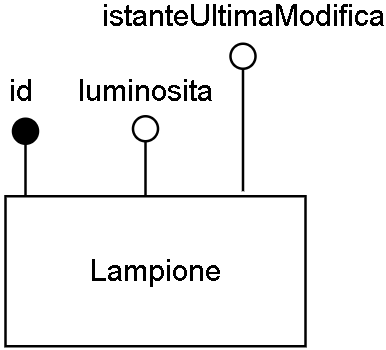
\includegraphics[width=4.5cm]{contenuti/specifica-basi-dati/img-sbd/coordinazione_concettuale.png}
\end{center}

\subsection{Progettazione logica}

\subsubsection{Schema concettuale ristrutturato - Schema Logico}

\begin{center}
    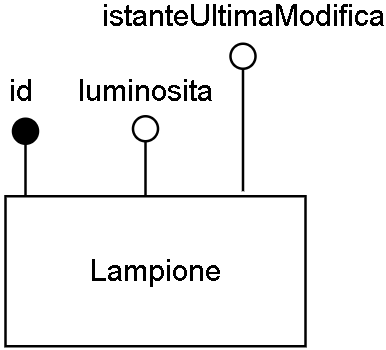
\includegraphics[width=4.5cm]{contenuti/specifica-basi-dati/img-sbd/coordinazione_logico.png}
\end{center}

\subsubsection{Descrizione schema relazionale}

Per questione di compatibilità con il DBMS alcuni nomi di attributi entità e relazioni sono stati normalizzati, utilizzando il camelCase, togliendo gli accenti, accorciando i nomi molto lunghi e con altre piccole accortezze.
La chiave primaria è indicata in \textbf{grassetto}, le chiavi esterne sono indicate con la \underline{sottolineatura}.

\textit{Lampione}(\textbf{id}, luminosita, lastSync)

\section{Base di dati sistema logging}

\subsection{Abstract}

L’obiettivo è sviluppare un servizio che tenga traccia in maniera intelligente dei log. Questo servizio offre numerosi benefici legati alla retrospettiva. Il miglioramento delle prestazioni del sistema, la risoluzione rapida dei problemi, il rilevamento delle minacce alla sicurezza e la generazione di informazioni utili per l'analisi e il miglioramento continuo sono solo alcuni dei benefici che questo servizio permette.

\subsection{Analisi dei requisiti}

\subsection{Progettazione concettuale}

\subsection{Progettazione logica}


\clearpage
\pagenumbering{Roman}
\listoffigures

\end{document}